\section{Aufgabe 2}
Nun wird eine Addiererschaltung entsprechend einer vorgegebenen Übertragungsfunktion aufgebaut. Anschließend wird experimentiert, welchen Einfluss die verschiedenen Bauteilwerte innerhalb des invertierenden Addierers und des invertierenden Verstärkers auf das Ausgangssignal haben.

\subsection{Methoden}
Nach den Vorgaben der Aufgabenstellung und den goldenen Regeln für den Operationsverstärker \cite{skript} gilt für den invertierenden Addierer:
\begin{equation}
U_{a}=-\,{\frac {10k\Omega }{10\,k\Omega +R_{8}}}\cdot\,U_{H}-\,{\frac {10k
\Omega}{10\,k\Omega +R_{10}}}\cdot\,U_{T}
\end{equation}
Dies bedeutet (bezogen auf Abbildung \ref{spicegesamt}):
\begin{equation}
R_{11}=R_{7}=R_{9}=10\si{k\Omega}
\end{equation}
Das Bauteilwerte der Wiederstände $R_{8}$ und  $R_{10}$ werden später noch verändert.
Dementsprechend wurde nun erstmals die gesamte Schaltung in Spice aufgebaut.\newline

\begin{figure}[h]
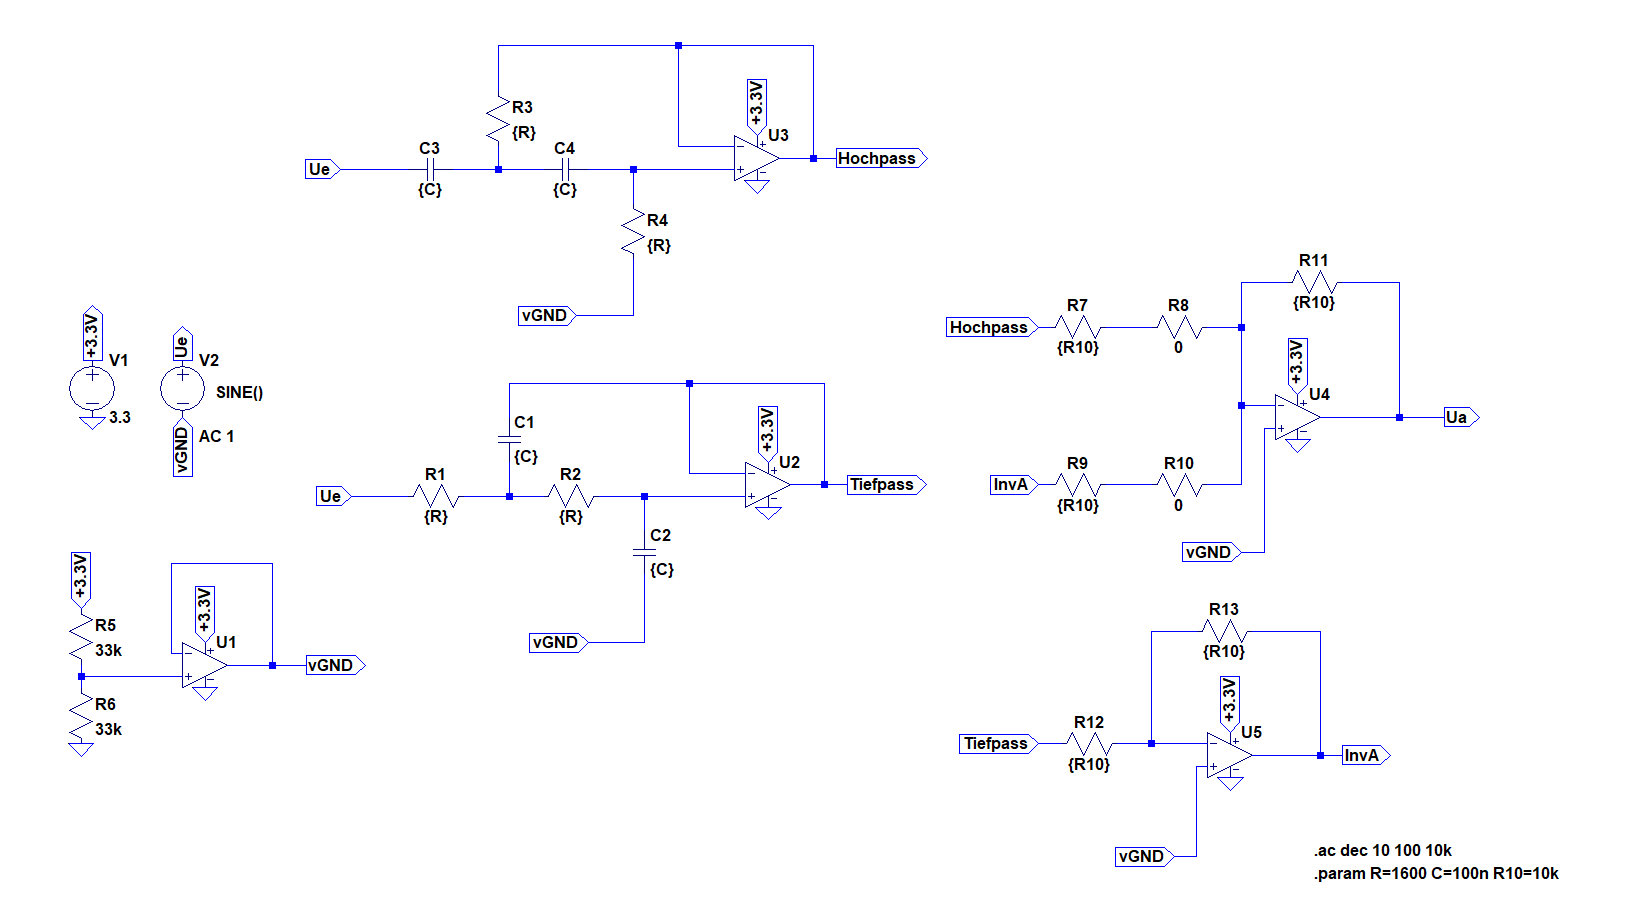
\includegraphics[width=14cm]{pics/SpiceSchaltungGesamt.png}
\caption{Der gesamte Schaltungsaufbau in LT Spice}
\label{spicegesamt}
\end{figure}

\newpage
Außerdem war es ebenfalls Teil der Aufgabe die Schaltung auf dem Breadbord nachzubauen und mit der LENLab Software auszumessen. Diese Bilder zeigen den Aufbau des \textbf{invertierenden Verstärker \ref{invV}} und des \textbf{invertierenden Addierers \ref{invA}.}

\begin{figure}[h]
\centering
\subfigure[]{
    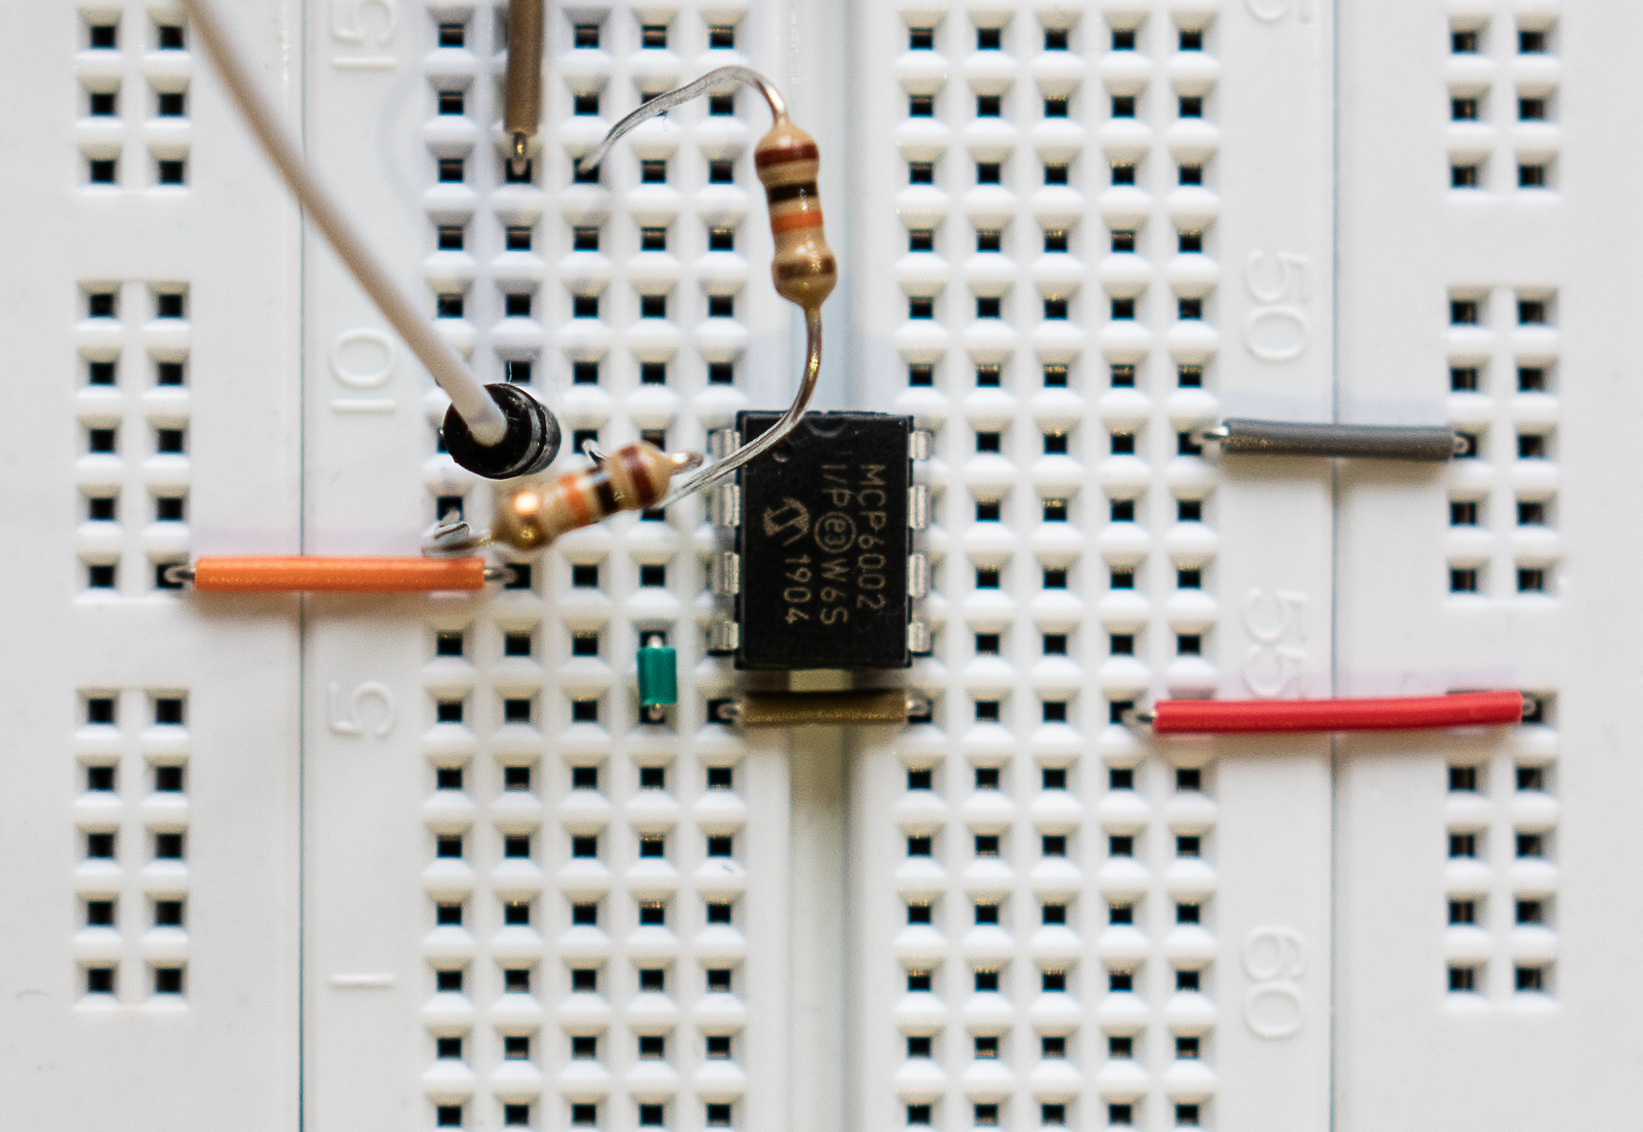
\includegraphics[width=6cm]{pics/Invertierer_aufgebaut.jpg}
  \label{invV}}
\subfigure[]{
  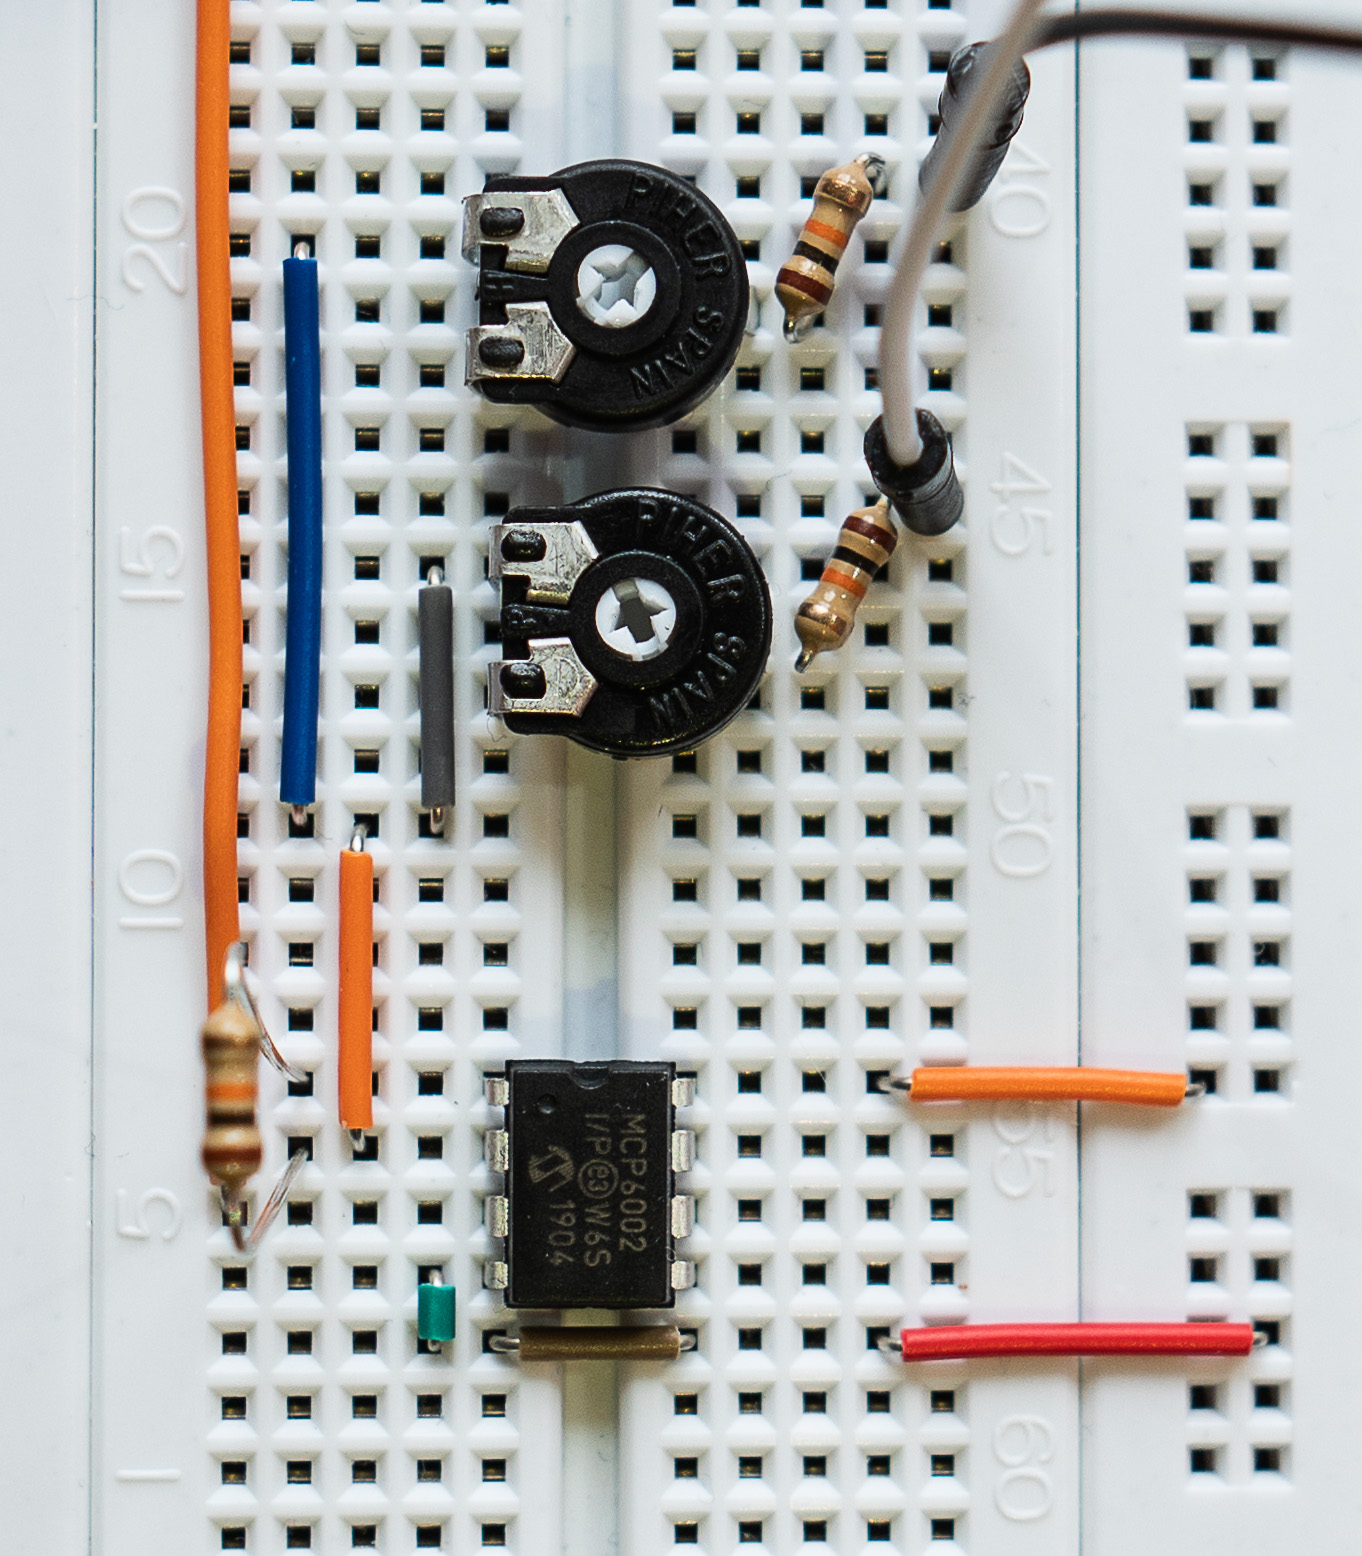
\includegraphics[width=4cm]{pics/Addierer_aufgebaut.jpg}
  \label{invA}}
\caption{Invertierender Verstärker (a) und Invertierender Addierer (b)}
\end{figure}

Zur Variation der Widerstände $R_{8}$ und $R_{10}$ wurde für diese Bauteile jeweils ein \newline Potentiometer($\sim 0-100k\Omega$) verbaut, wie es in Abbildung \ref{invA} zu sehen ist.
\newline Sowohl mit dem Schaltungsaufbau in Spice als auch mit der auf dem Breadboard werden Messungen durchgeführt. Deren Ergebnisse im Folgenden vorgestellt werden.

\subsection{Ergebnisse}
% A)Simulieren Sie für Werte von R1 = R2 = 0Ω ein Bodediagramm der Gesamtschaltung zwischen 100Hz und 10kHz.
\subsubsection{Aufgabe A}
\label{A}
Simulation eines Bodediagramms der Gesamtschaltung zwischen $\si{100}{Hz}$ und $\si{10}{kHz}$.
\newline $R_{8}$ und $R_{10}$ betragen hierbei $\si{0}{\Omega}$.
\begin{figure}[h]
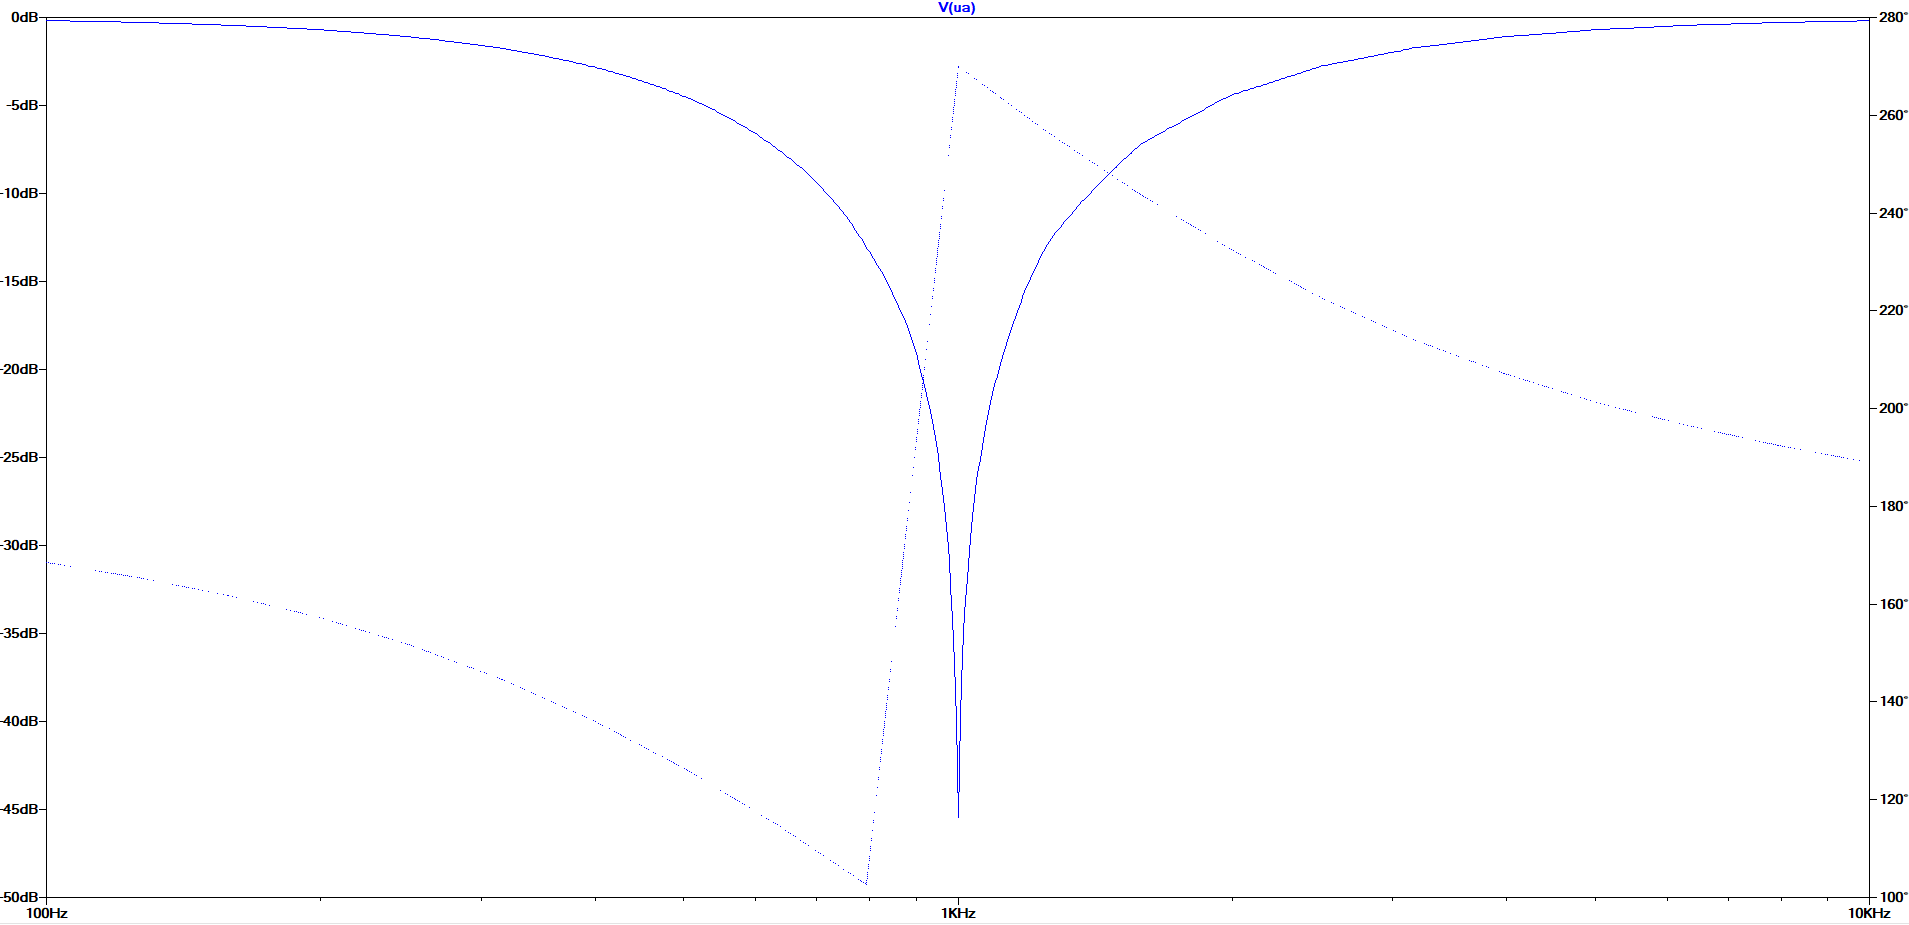
\includegraphics[width=14cm]{pics/BodeAd_ohneInv}
\caption{Das Bodediagramm der Gesamtschaltung ohne invertierenden Verstärker}
\label{bodeA}
\end{figure}

% B) Wie erklären Sie sich den Einbruch des Amplitudengangs bei der Grenzfrequenz Ihrer Filterschaltungen?

% C) Fügen Sie zwischen Tiefpass und Addierschaltung einen invertierenden Verstärker mit Verstärkungsfaktor 1 ein und wiederholen Sie die Simulation aus a). Was beobachten Sie nun? Wie nennt sich ein Filter, welches das beobachtete Übertragungsverhalten aufweist?
\subsubsection{Aufgabe C}
\label{C}
Es wird ein invertierender Verstärkerr zwischen den Ausgang des Tiefpasses und der Addiererschaltung eingebaut. Die Simulation des Bodediagramms der Gesamtschaltung wird wiederholt. $R_{8}$ und $R_{10}$ betragen immernoch $\si{0}{\Omega}$.
\begin{figure}[h]
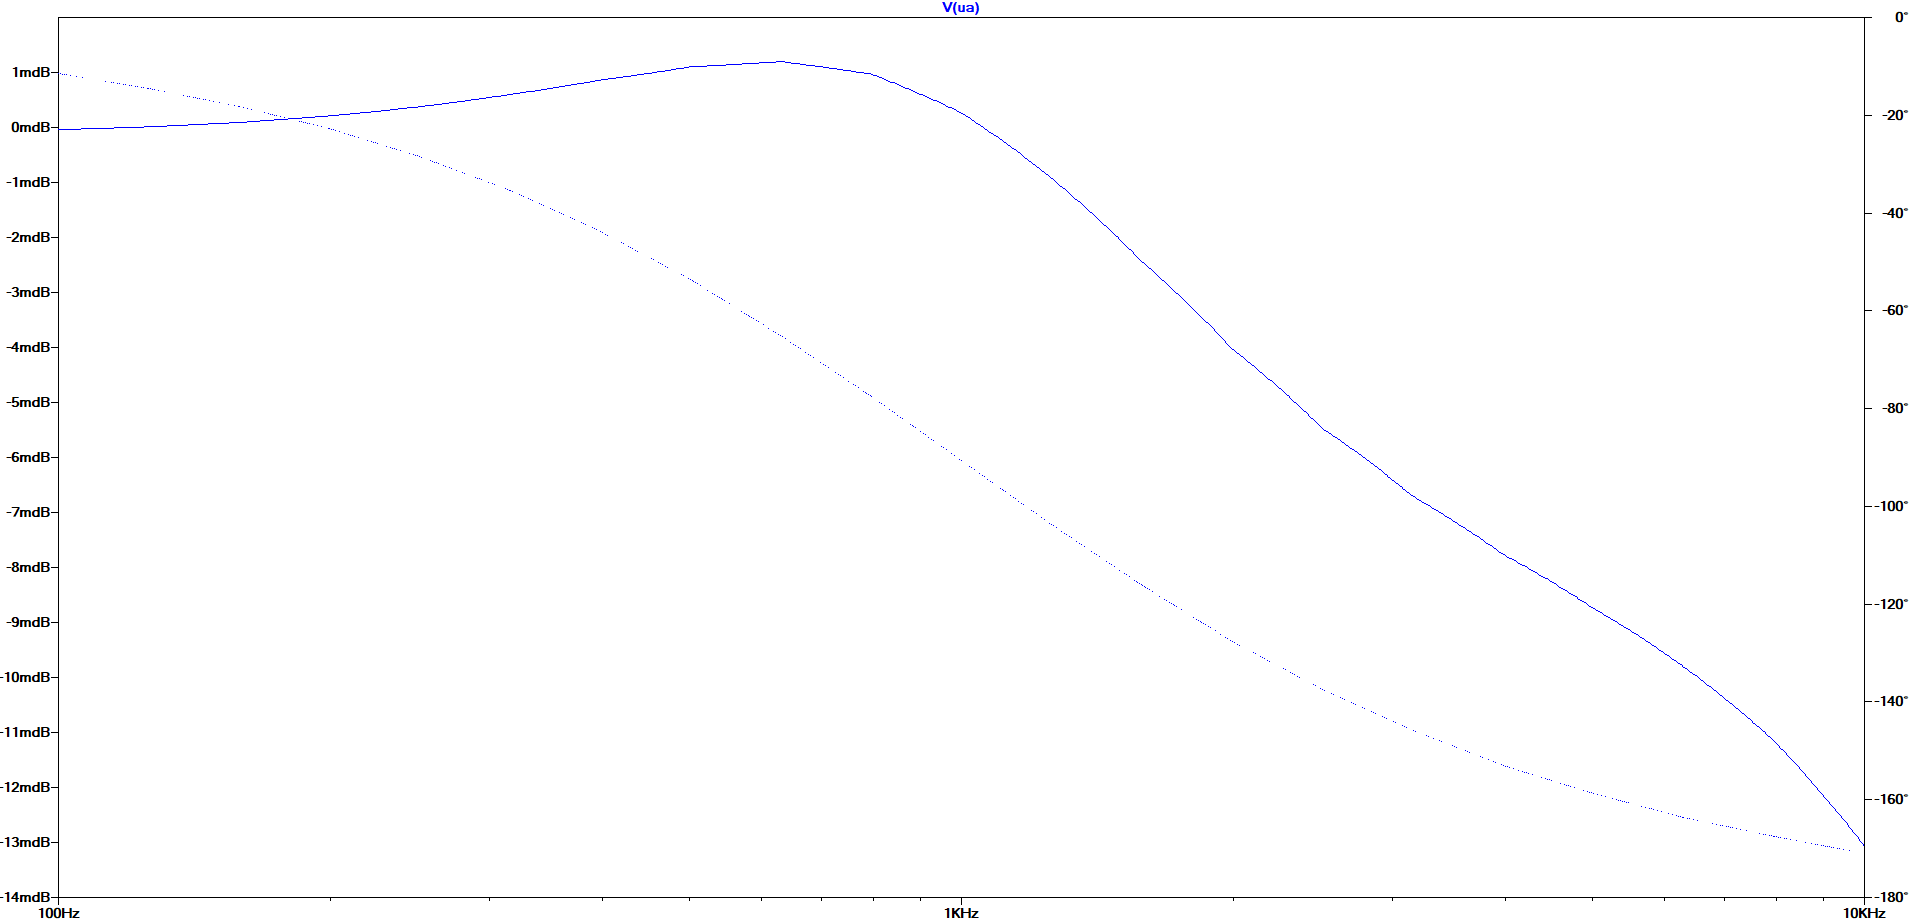
\includegraphics[width=14cm]{pics/BodeAd_mitInv}
\caption{Das Bodediagramm der Gesamtschaltung mit invertierenden Verstärker}
\label{bodeC}
\end{figure}

% D) Simulieren Sie weitere Bodediagramme der Gesamtschaltung für (R1 = 10kΩ, R2 = 90kΩ) und (R1 = 90kΩ, R2 = 10kΩ)
\subsubsection{Aufgabe D}
\label{D}
Es werden weitere Bodediagramme simuliert. Nun werden die Werte für $R_{8}$ und $R_{10}$ entsprechend der Bildbeschriftung variiert.
\begin{figure}[h]
\subfigure[Bodediagramm für $R_{8}=\si{10}{\,k\Omega}$ und \newline $R_{10}=\si{90}{\,k\Omega}$]{
  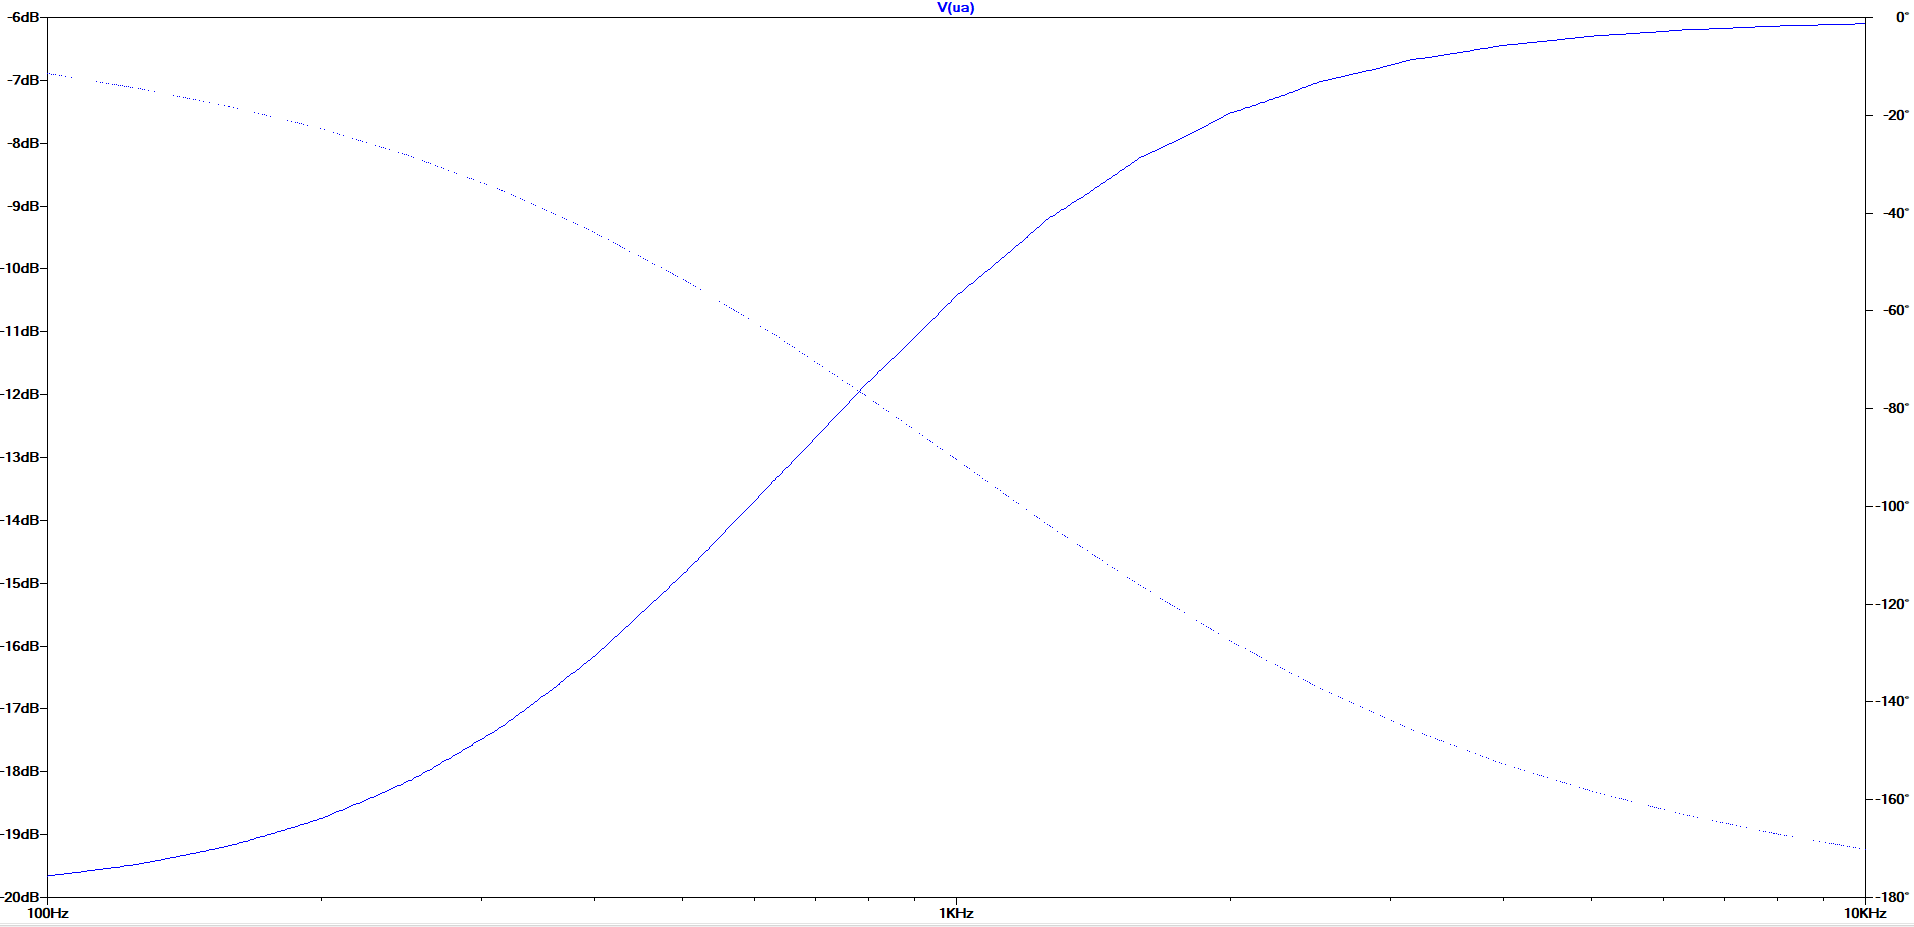
\includegraphics[width=0.48\textwidth]{pics/10_90}
  \label{Bode1090}}
\subfigure[Bodediagramm für $R_{8}=\si{90}{\,k\Omega}$ und \newline $R_{10}=\si{10}{\,k\Omega}$]{
  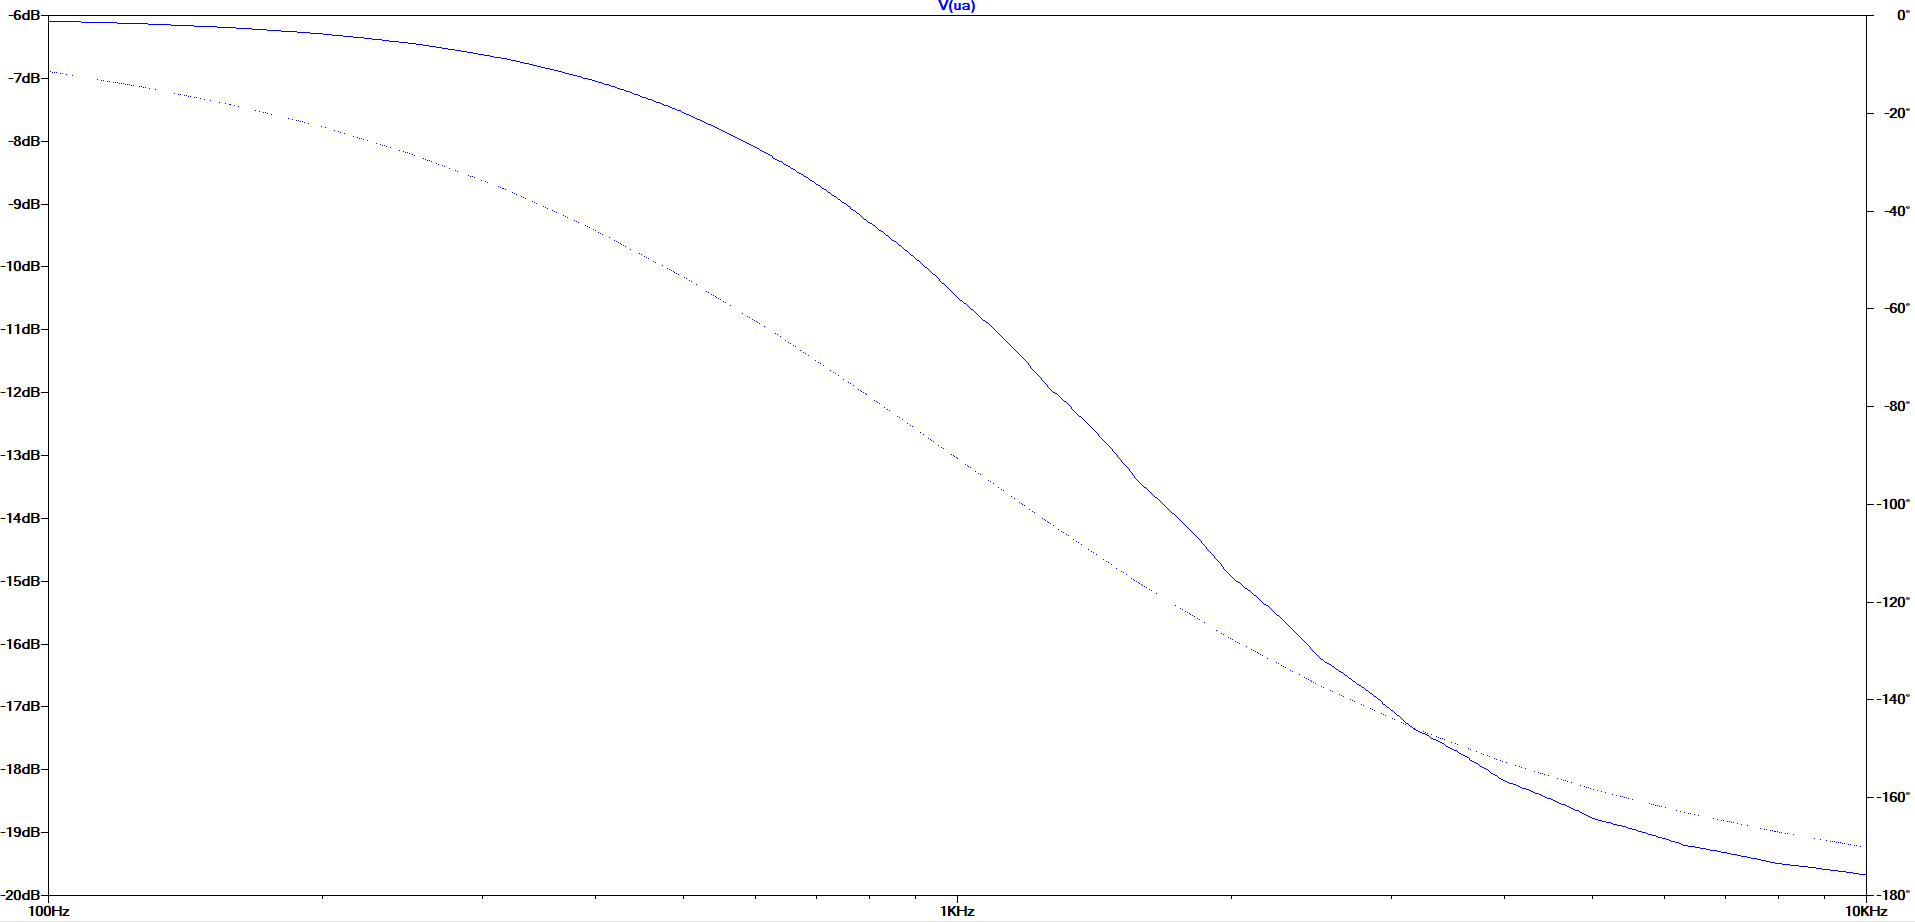
\includegraphics[width=0.48\textwidth]{pics/90_10}
  \label{Bode9010}}
\caption{Bodediagramme für Gesamtschaltung mit variierten Bauteilwerten}
\end{figure}

% E)Bauen Sie die Addierschaltung inklusive invertierendem Verstärker jetzt auch auf Ihrem Steckbrett auf. Verwenden Sie für die Widerstände R1 und R2 die beiden Potentiometer (0...100kΩ)desBauteilsortiments.FührenSieBodediagramm-Messungen derGesamtschaltung für R1 = R2 = 0Ω und bei ein paar weiteren Poti-Einstellungen durch.
\newpage
\subsubsection{Aufgabe E}
\label{E}
Die gesamte Schaltung wurde nun auf dem Steckbrett aufgebaut. Hierbei wurde für $R_{8}$ und $R_{10}$ jeweils ein Potetiometer verbaut. Somit lassen sich die beiden Widerstände stufenlos zwischen $\si{0}{\Omega}$ und $\si{100}{k\Omega}$ verändern. Es folgen sechs Bodediagramm-Messungen mit den angegebenen Bauteilwerten. In \textcolor{blue}{blau ist die Amplitude} und in \textcolor{red}{rot die Phase} aufgetragen. Ein exaktes Einstellen der Potentiometer ist nicht möglich, deshalb werden die Widerstände hier nur gerundet angegeben.

\begin{figure}[h]
\centering
\subfigure[Bodediagramm für $R_{8}\approx \si{0}{\Omega}$, $R_{10}\approx \si{0}{\Omega}$]{
  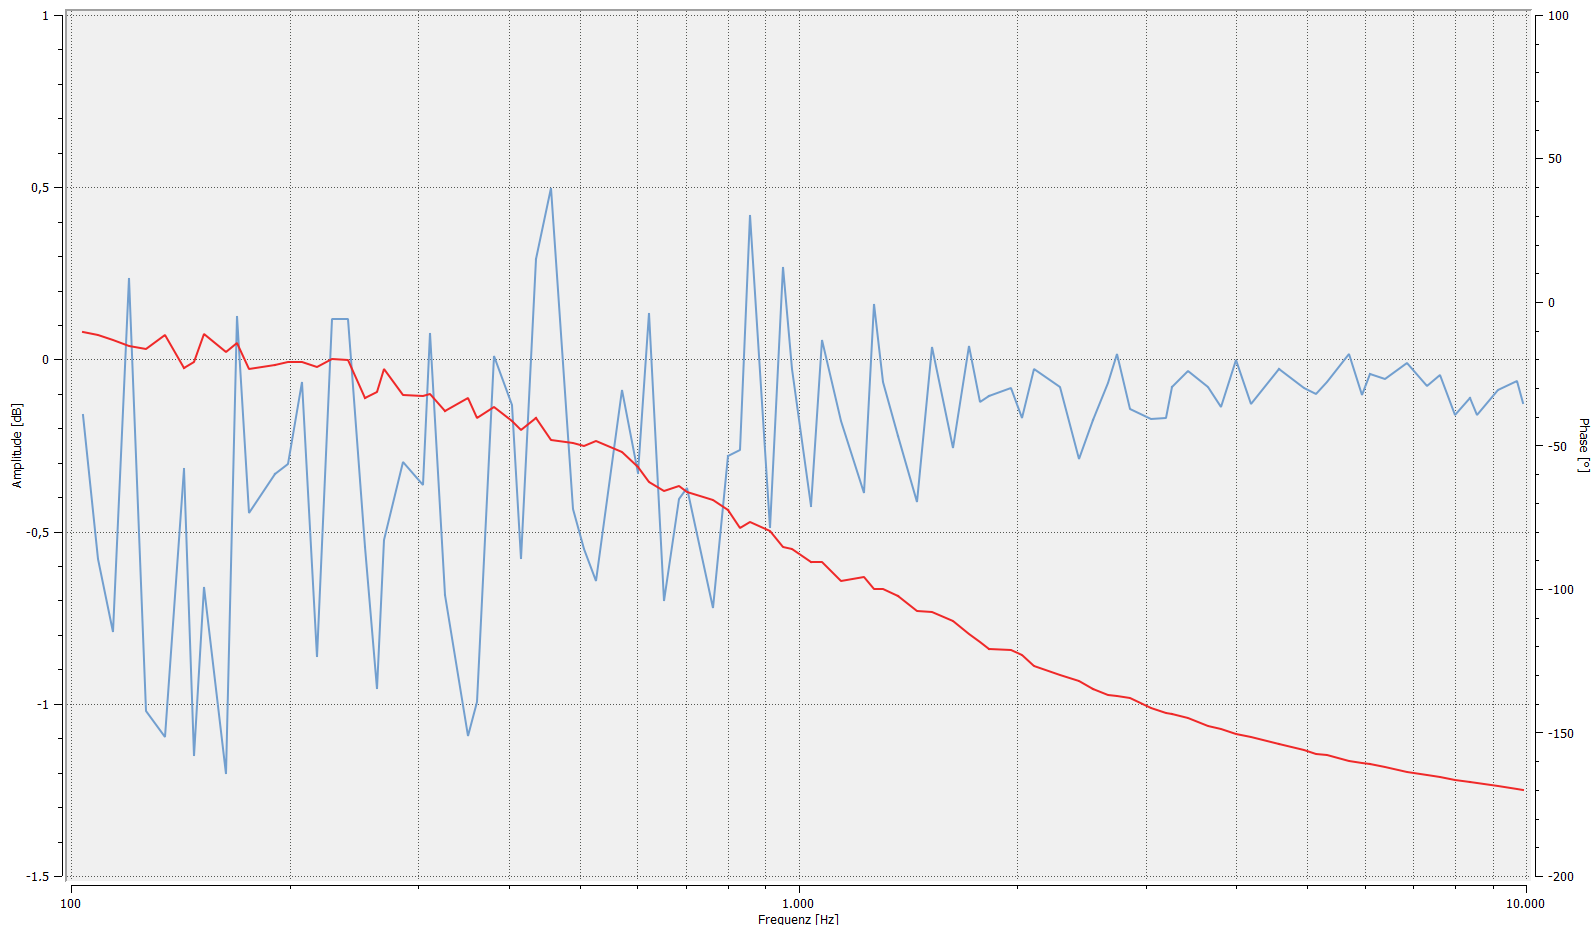
\includegraphics[width=8cm]{pics/0_0Steckbrett}
  \label{0_0SB}}%
\subfigure[Bodediagramm für $R_{8}\approx \si{100}{\,k\Omega}$,$R_{10}\approx \si{100}{\,k\Omega}$]{
  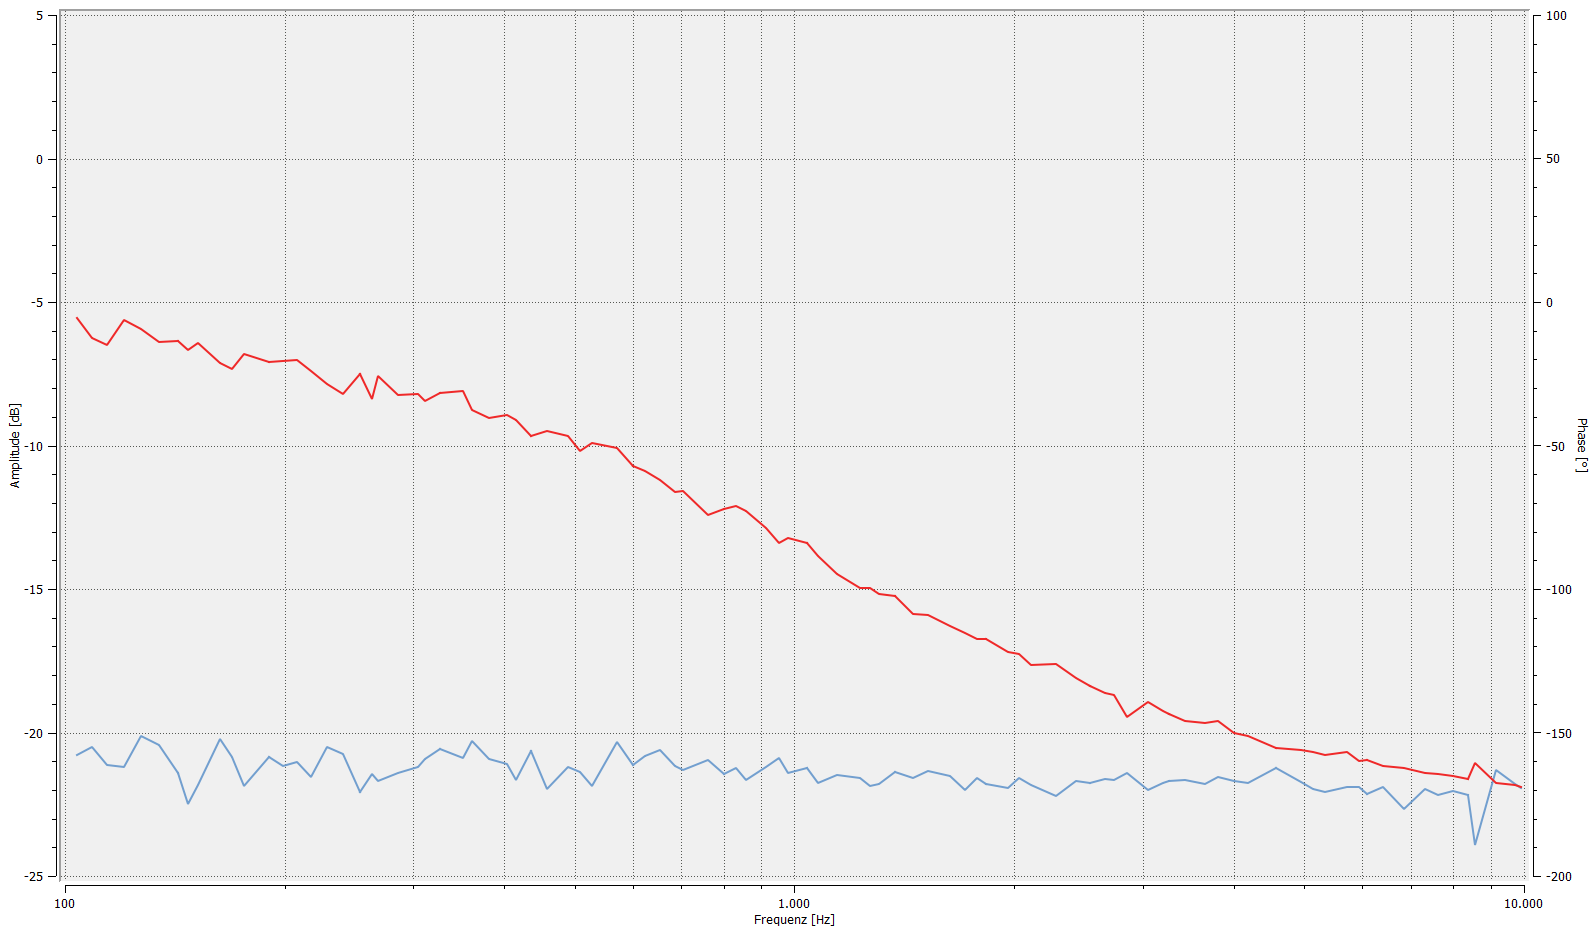
\includegraphics[width=8cm]{pics/100_100Steckbrett}
  \label{1_1SB}}
\subfigure[Bodediagramm für $R_{8}\approx \si{0}{\Omega}$, $R_{10}\approx \si{100}{\,k\Omega}$]{
  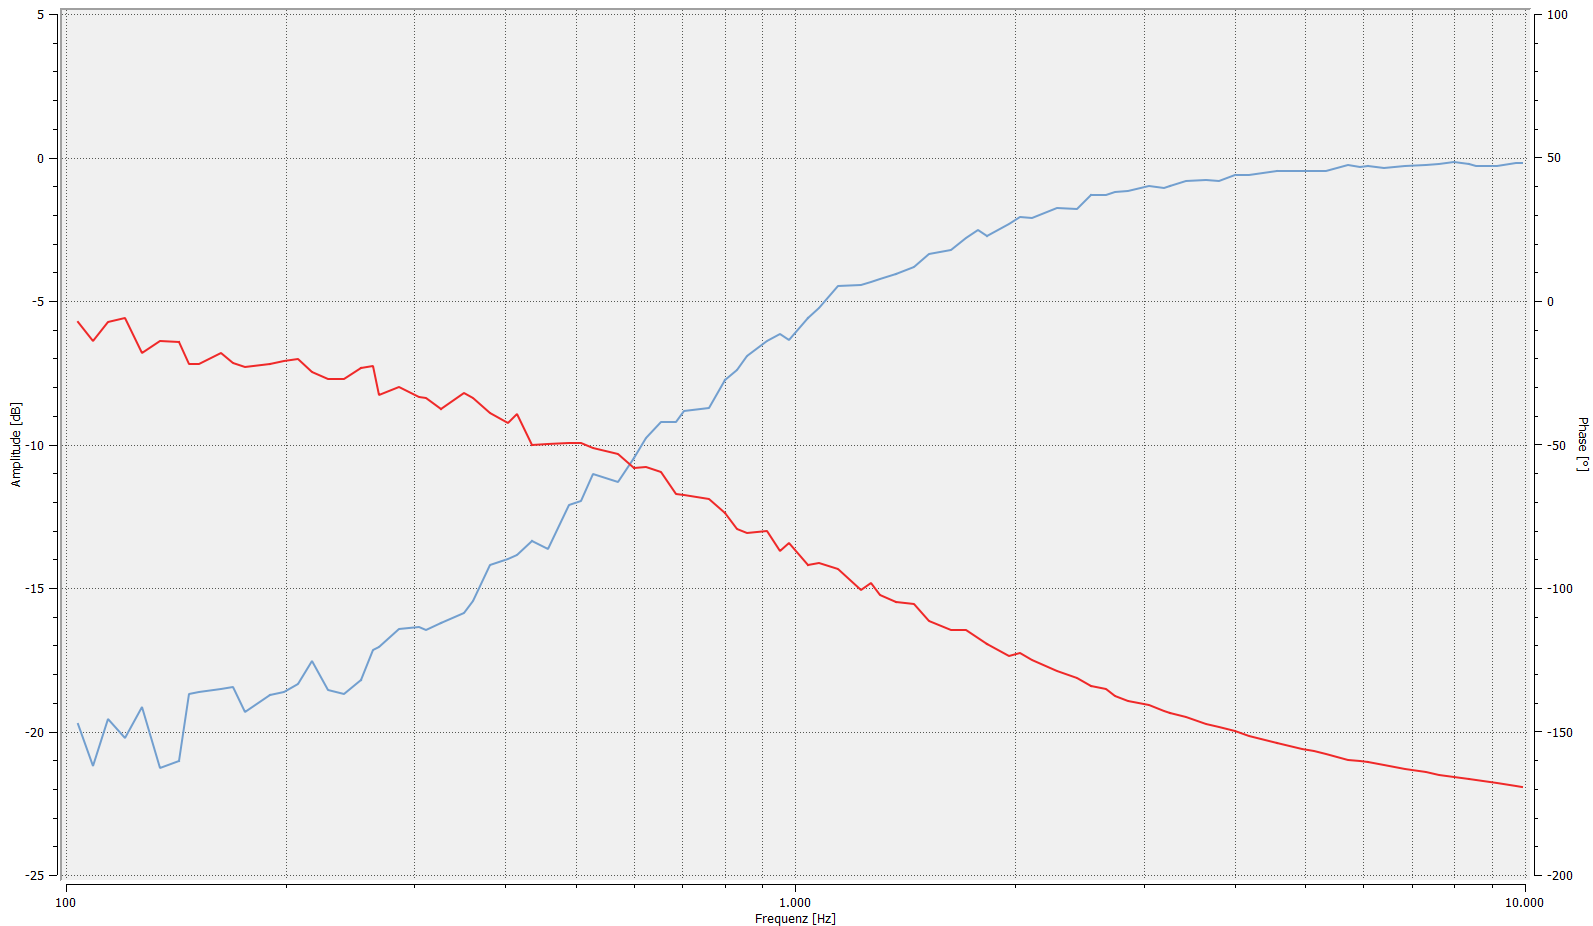
\includegraphics[width=8cm]{pics/0_100Steckbrett}
  \label{0_1SB}}%
\subfigure[Bodediagramm für $R_{8}\approx \si{100}{\,k\Omega}$, $R_{10}\approx \si{0}{\Omega}$]{
  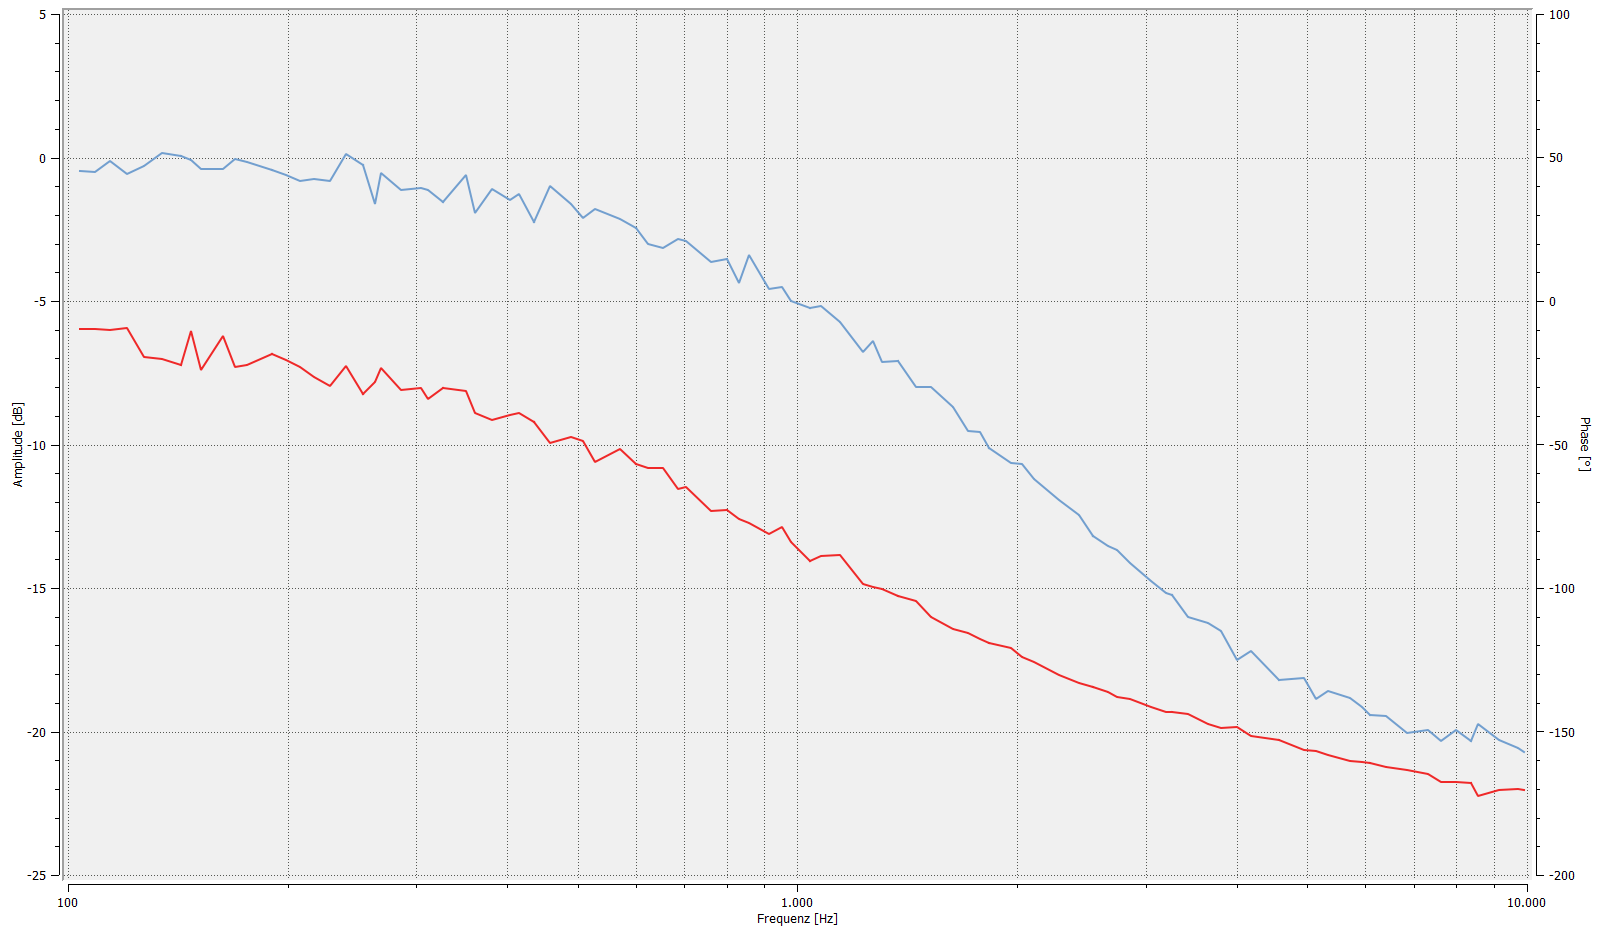
\includegraphics[width=8cm]{pics/100_0Steckbrett}
  \label{1_0SB}}
\subfigure[Bodediagramm für $R_{8}\approx \si{30}{\,k\Omega}$, $R_{10}\approx \si{60}{\,k\Omega}$]{
  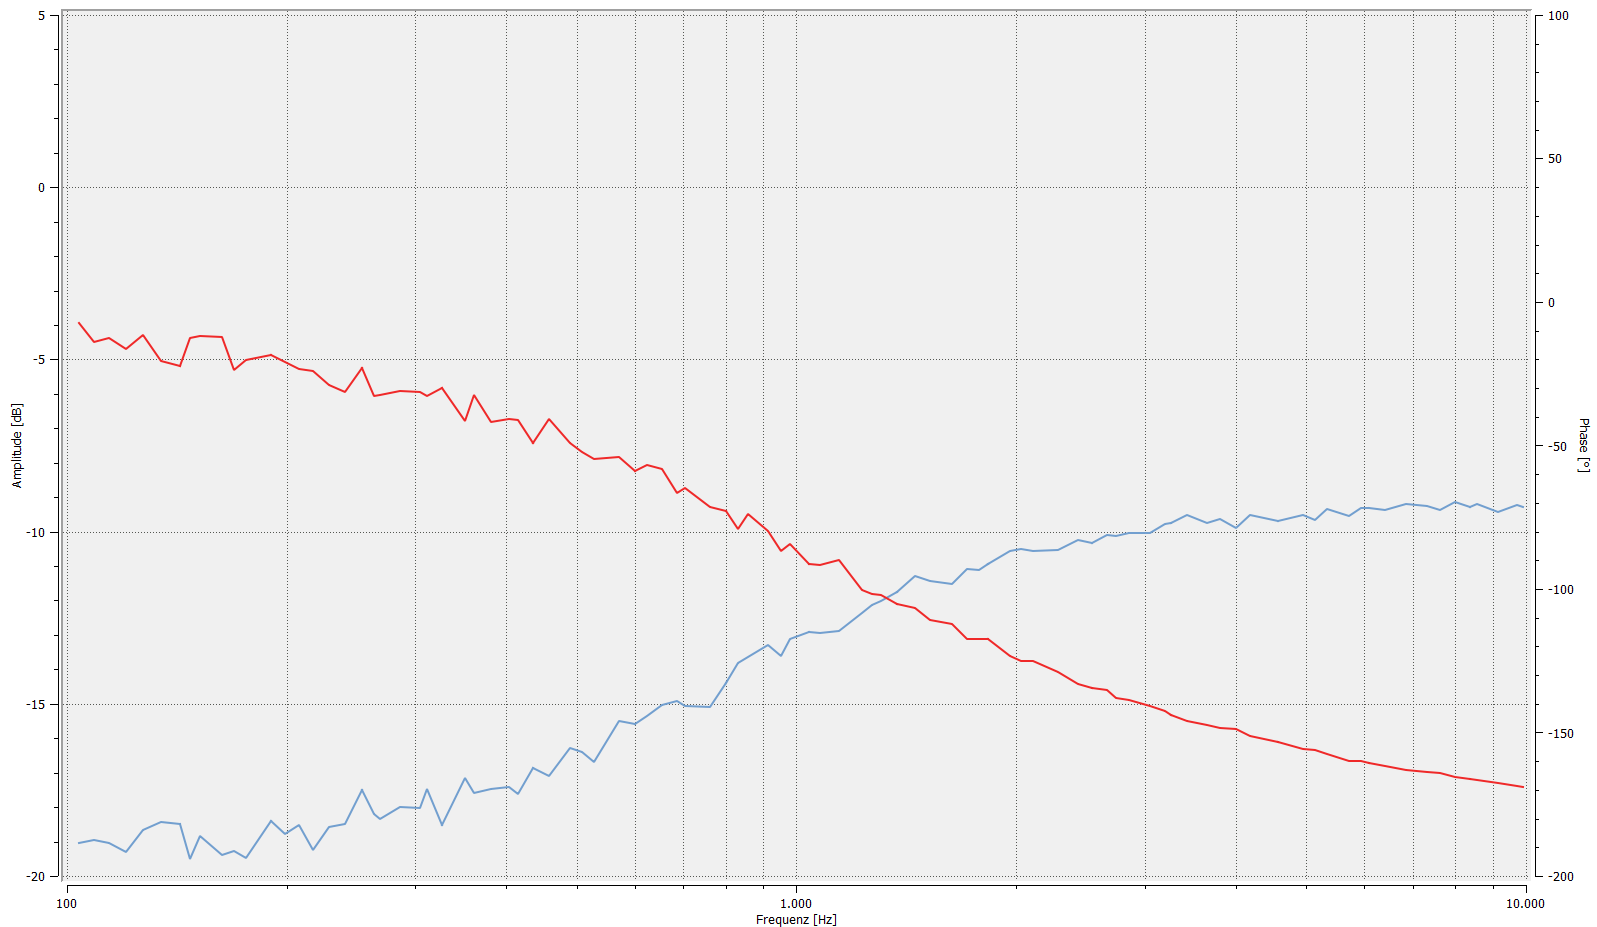
\includegraphics[width=8cm]{pics/30_60Steckbrett}
  \label{3_6SB}}%
\subfigure[Bodediagramm für $R_{8}\approx \si{60}{\,k\Omega}$, $R_{10}\approx \si{30}{\,k\Omega}$]{
  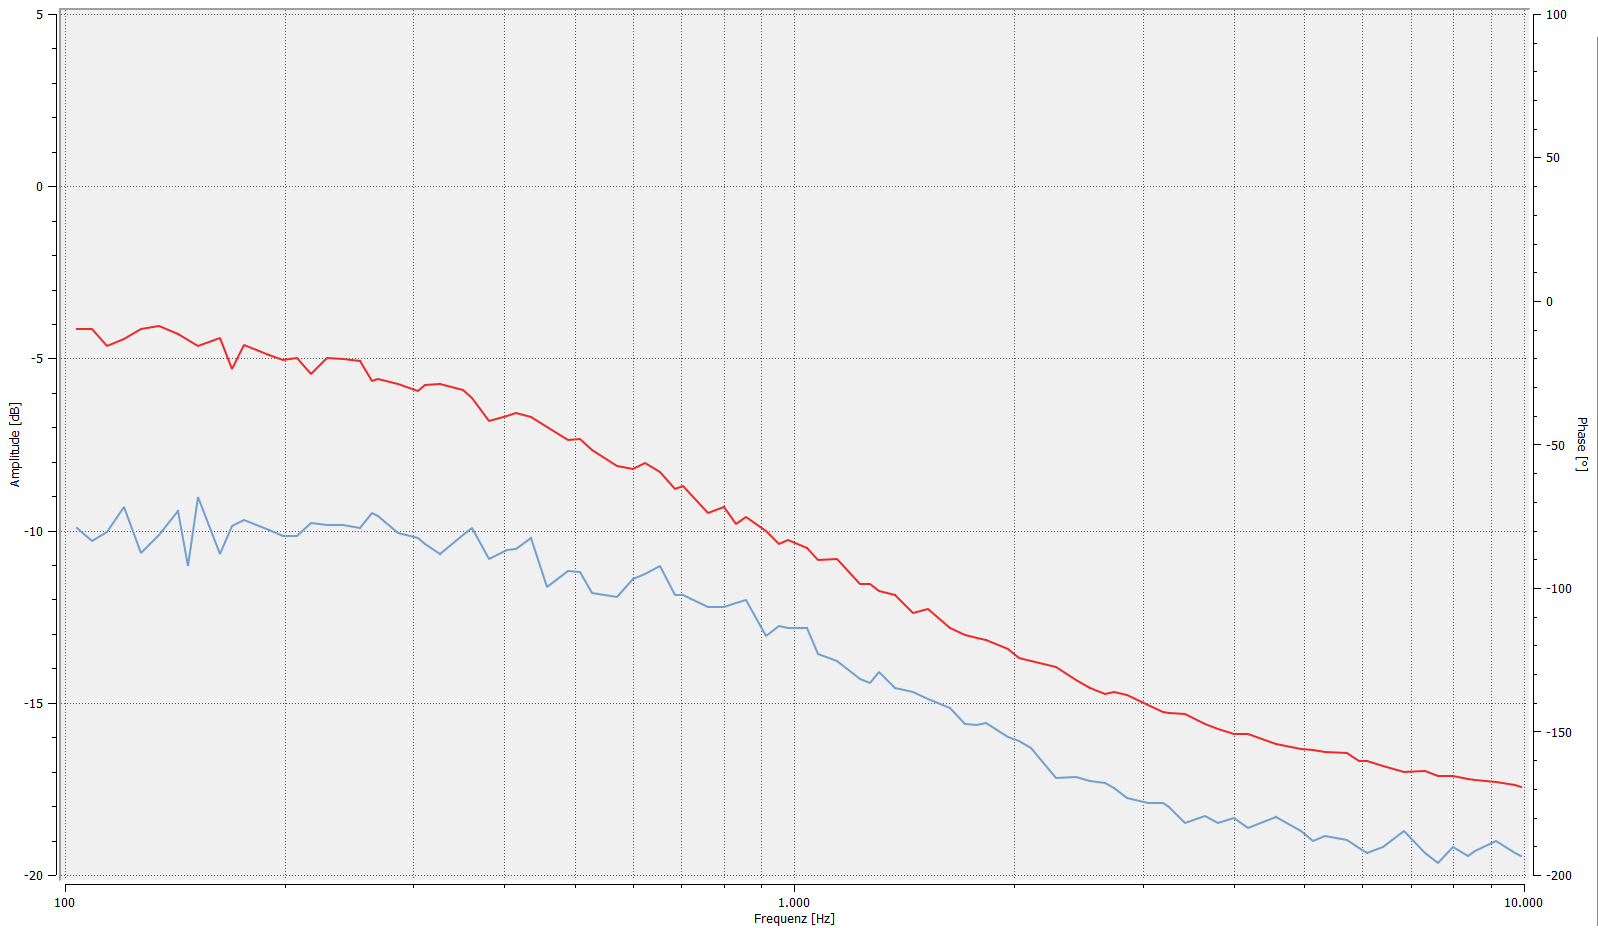
\includegraphics[width=8cm]{pics/60_30Steckbrett}
  \label{6_3SB}}
\caption{Bodediagramme für Gesamtschaltung mit Potentiometer von $R_{8}$ und $R_{10}$}
\end{figure}
\newpage
% F)  Nun sollen zwei Sinussignale verschiedener Frequenz überlagert und auf den Eingang des Equalizers gegeben werden. Nutzen Sie zur Überlagerung die gleiche Schaltung wie in Abbildung 4, jedoch mit Kanal A und Kanal B des DAC an den beiden Enden des Spannungsteilers.ErzeugenSiemitdemSignalgeneratoranKanalAeineFrequenzvon ca. 250Hz. An Kanal B soll ein Sinus mit ca. 5kHz ausgegeben werden. Dies erreichen Sie, indem Sie einen Frequenzmultiplikator für Kanal B von 20 einstellen. Nehmen Sie mit dem Oszilloskop das Eingangssignal und die Ausgangssignale bei den beiden Extremstellungen auf (R1 = 0Ω, R2 = 100kΩ und umgekehrt).

\subsubsection{Aufgabe F}
\label{F}
Zwei sich überlagernde Sinussignale mit den Frequenzen $\si{250}{Hz}$ und $\si{5}{\,k\Omega}$ werden in die Steckbrettschaltung hinein geschickt. Es wird das \textcolor{blue}{Eingangssignal in blau} und das \textcolor{red}{Ausgangssignal in rot} jeweils für die Einstellungen $R_{8}=\si{0}{\Omega}$, $R_{10}=\si{100}{\,k\Omega}$ und $R_{8}=\si{100}{\,k\Omega}$, $R_{10}=\si{0}{\Omega}$ aufgezeichnet.

\begin{figure}[h]
\centering
\subfigure[Oszilloskop für $R_{8}=\si{0}{\Omega}$ und $R_{10}=\si{100}{\,k\Omega}$]{
  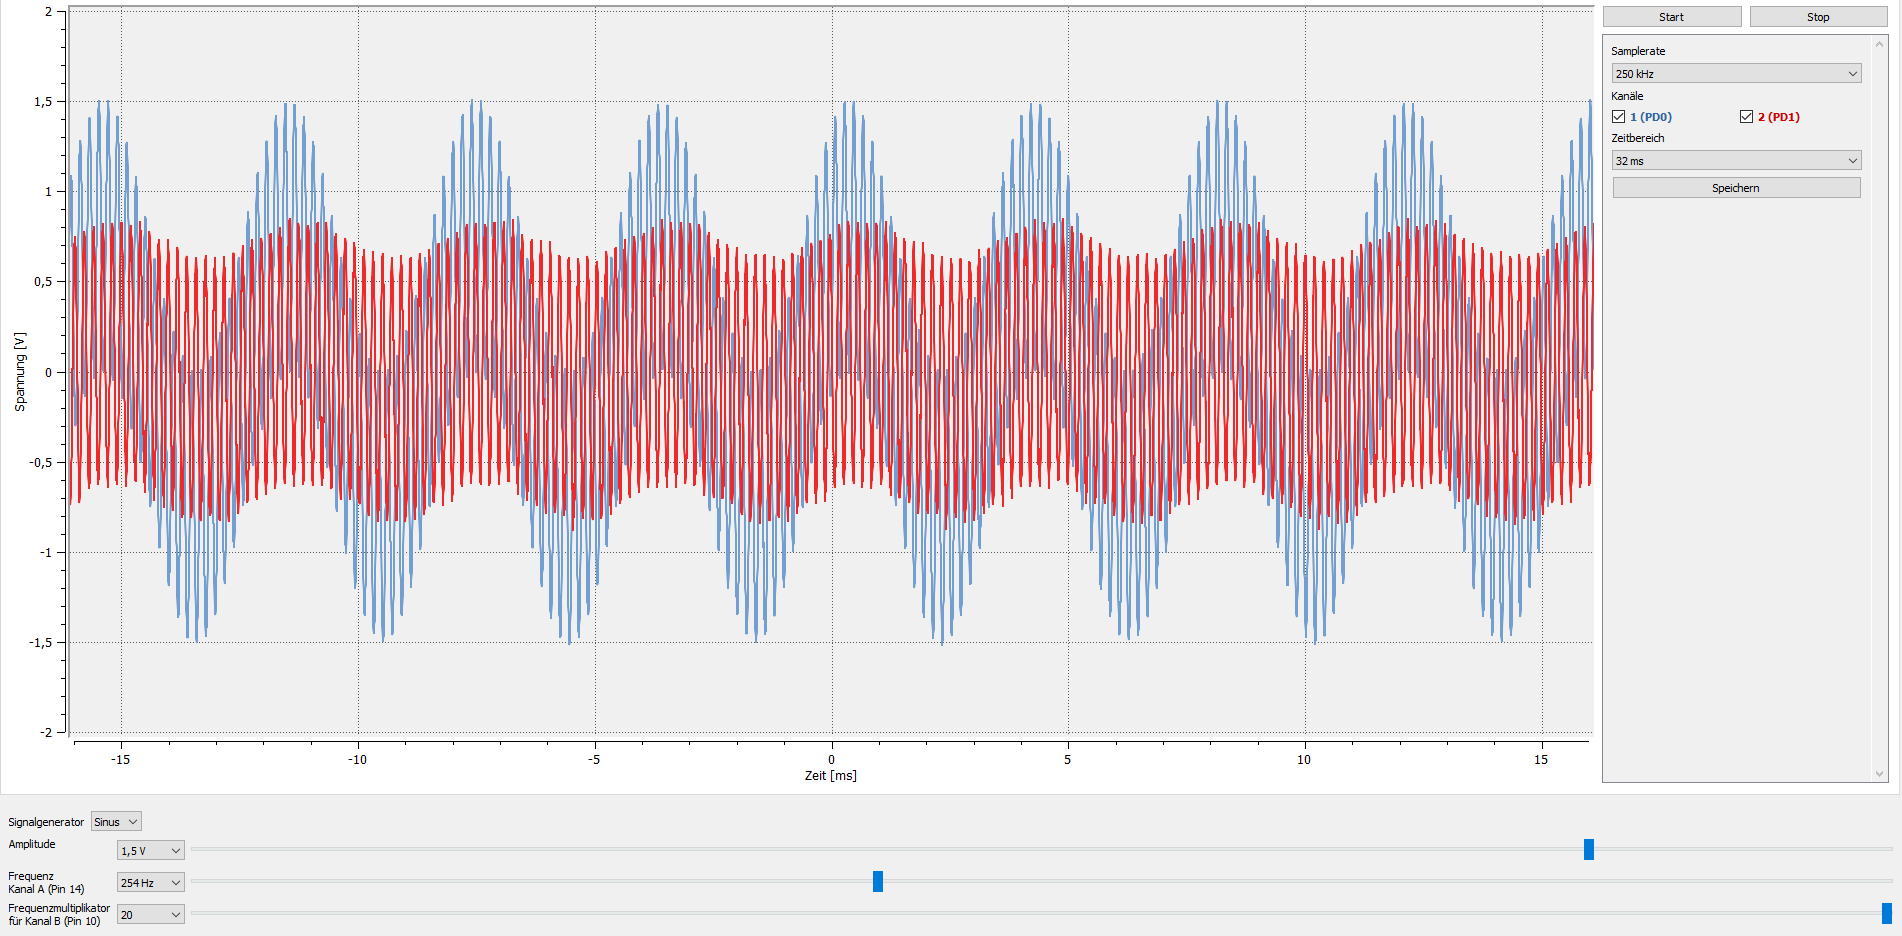
\includegraphics[width=17cm]{pics/3.3f_0_100}
  \label{sin0_1}}
\subfigure[Oszilloskop für $R_{8}=\si{100}{\,k\Omega}$ und $R_{10}=\si{0}{\Omega}$]{
  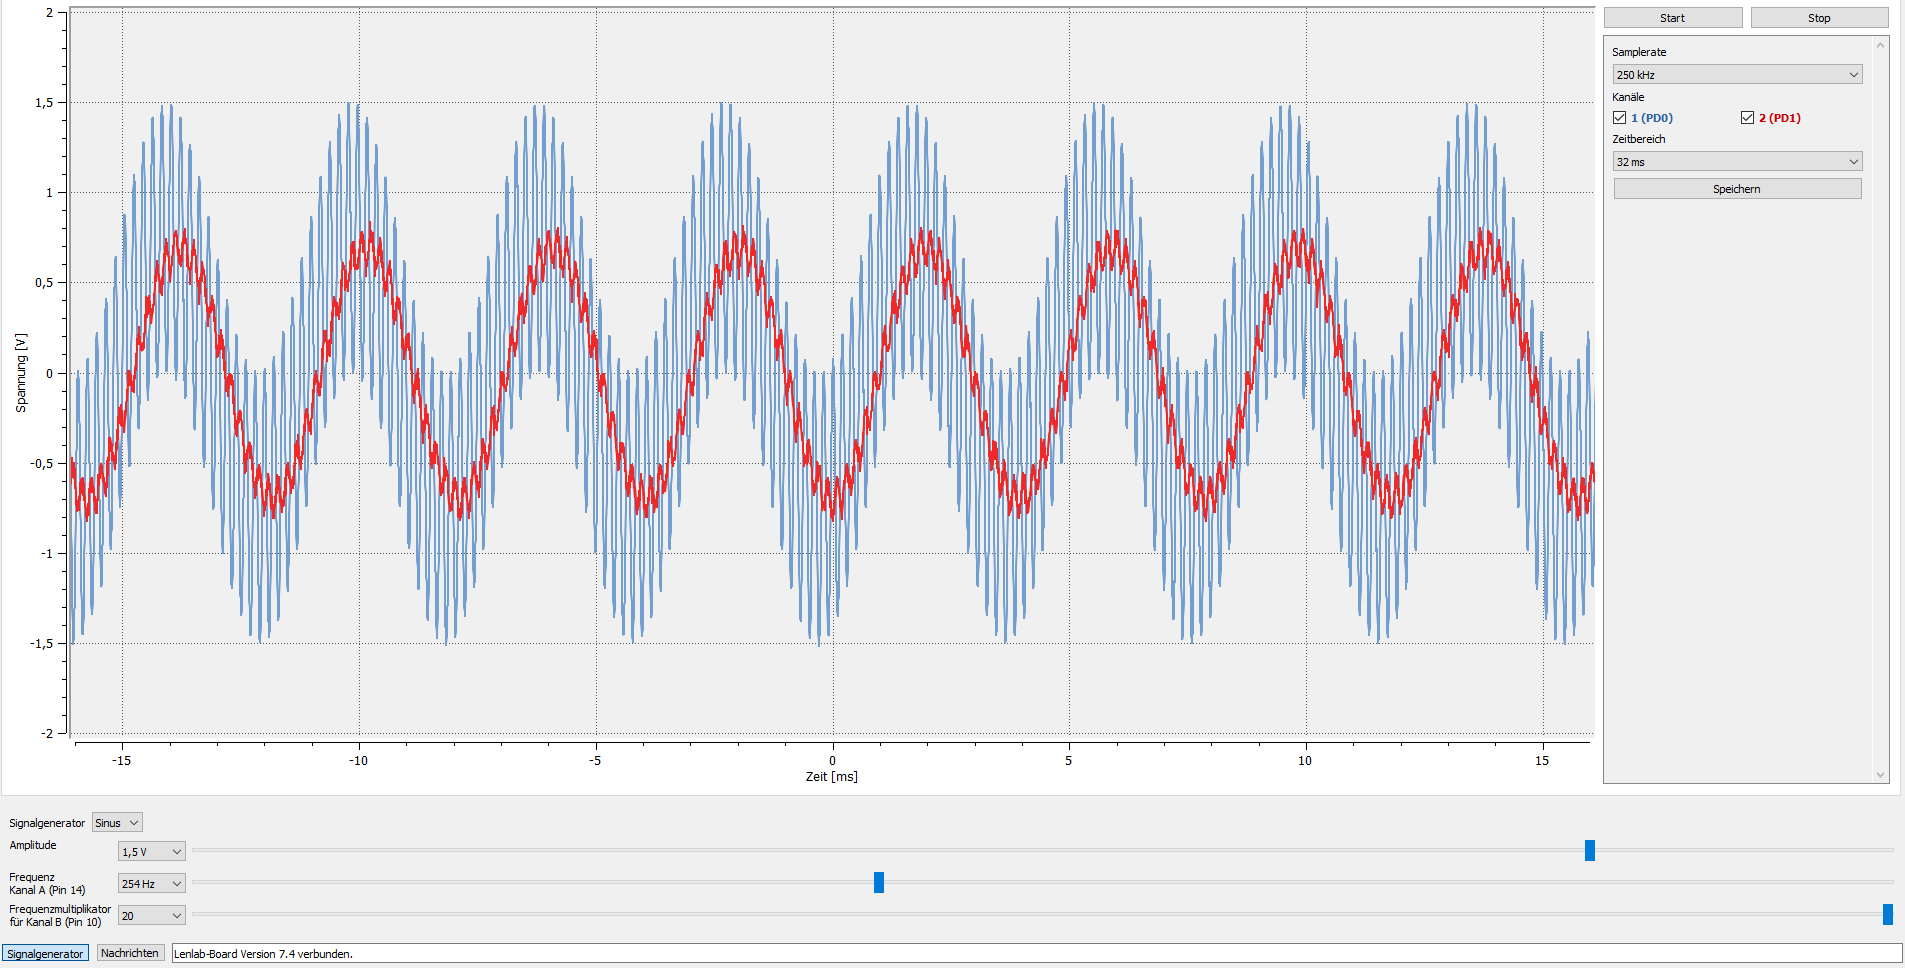
\includegraphics[width=17cm]{pics/3.3f_100_0}
  \label{sin1_0}}
\caption{Oszilloskop für Sinussignal}
\end{figure}


\newpage
\subsection{Diskussion}
\subsubsection{Diskussion von Aufgabe A + B[\ref{A}]}
Es werden die Signale des Hoch- und Tiefpassfilters addiert. Der Einschnitt in der Mitte, den man im ersten Moment durch die Addition von $2\cdot \si{-6}{dB}$ (Filter 2. Ordnung bei Grenzfrequenz) für erklärbar hält, ist bei genauerem Hinsehen mit $\si{45}{dB}$ dann doch etwas zu tief. Zusätzlich spielt hier nämlich noch eine zweite Begebenheit eine wichtige Rolle. Während der Tiefpassfilter zweiter Ordnung die Phase seines Signals um genau $\si{-90}{^{\circ}}$ dreht, dreht der Hochpassfilter zweiter Ordnung die Phase seines Signals um $\si{+90}{^{\circ}}$. Somit sind die zu addierenden Signale genau um $\si{180}{^{\circ}}$ phasenverschoben. Unterscheiden sich die Amplituden der phasenverschobenen Signale deutlich, so fällt diese destruktive Interferenz kaum ins Gewicht. An der Grenzfrequenz betragen die Amplituden aber beide ca.$\si{-6}{dB}$. Deshalb heben sich die beiden Signale an der Grenzfrequenz gegenseitig komplett auf. Dadurch entsteht der charakteristische Einschnitt in Abbildung \ref{bodeA}.

\subsubsection{Diskussion von Aufgabe C [\ref{C}]}
Um den ungewollten Einschnitt im Bodediagramm der Aufgabe A [\ref{A}] zu vermeiden, wird nun ein invertierender Verstärker mit einer Verstärkung von 1 zwischen den Tiefpassfilter und die Addiererschaltung gesetzt. Dieser Verstärkt das Signal nicht, sondern hat lediglich die Aufgabe die Phase des Tiefpasssignals um $\si{180}{^{\circ}}$ zu drehen. Addiert man nun die beiden Signale von Hochpassfilter und invertierendem Verstärker zusammen, so erhält man das Bodediagramm auf Abbildung \ref{bodeC}.
Dieses vermittelt zuerst den Eindruck die Gesamtschaltung würde jetzt eine Art Bandpass-Charakteristik haben. Die Skala des Diagramms \ref{bodeC} verrät allerdings, dass hier nur eine minimale Dämpfung vorliegt. Die folgende Abbildung zeigt deutlich,

\begin{figure}[h]
\centering
\includegraphics[width=13cm]{pics/Bode_vergleich}
\caption{Bodediagramm für \textcolor{blue}{Ausgangssignal}, \textcolor{green}{Tiefpasssignal}, \textcolor{red}{Hochpasssignal}}
\label{vergleich}
\end{figure}

dass die in Abbildung \ref{bodeC} gezeigten Dämpfungen in Relation zur Dämpfung, die am Hochpass- und Tiefpassfilter vorliegt, zu vernachlässigen sind.
\newpage
\subsubsection{Diskussion von Aufgabe D [\ref{D}]}
\label{DiskussionD}
Die beiden in LT Spice simulierten Kurven \ref{Bode1090} und \ref{Bode9010} zeigen wie der 2 Band Equalizer eingesetzt wird. Mit verscheiden großen Widerständen vor dem Hochpass- und Tiefpasseingang des Addierer wird das Mischverhältnis des beiden Signale bestimmt. Für die Simulation in Abbildung \ref{Bode1090} wurde das Signal kommend vom Tiefpassfilter mit einem deutlich höheren Widerstand ($\si{90}{\,k \Omega}$) gehemmt als jenes, welches vom Hochpass kommt ($\si{10}{\,k\Omega}$). Für die Zweite Simulation (\ref{Bode9010}) wurden die Werte von $R_{8}$ und $R_{10}$ lediglich vertauscht. Entsprechend ist der Verlauf der Amplitude hier symmetrisch zum Verlauf der ersten Kurve.\newline Das Verhältnis von hochfrequenten und niederfrequenten Signalanteilen lässt sich also über diese simple Einstellung der Widerstände einstellen.

\subsubsection{Diskussion von Aufgabe E [\ref{E}]}
Um die in \ref{DiskussionD} angesprochene Anpassung der Widerstände auf dem Steckbrett zu realisieren wurden Potentiometer verbaut. Somit ist eine stufenlose Einstellung von $R_{8}$ und $R_{10}$ zwischen $\si{0}{\Omega}$ und $\si{100}{k\Omega}$ möglich. Die sechs Bodedigramme aus Kapitel \ref{E} zeigen, dass die Bestimmmung des Mischverhältnisses nicht nur in der Simulation funktioniert. Abbildung \ref{0_0SB} zeigt das Mischverhältnis bei $R_{8}\approx \si{0}{\Omega}$, $R_{10}\approx \si{0}{\Omega}$. Die Amplitude sollte somit konstant sein. Die Skala des Bodediagramms \ref{0_0SB} zeigt, dass die zu beobachtenden Schwankungen sich nur im Bereich $\si{-1}{-}{+0,5}{dB}$ abspielen und somit zu vernachlässigen sind.
In Abbildung \ref{1_1SB} ist zu beobachten, dass bei $R_{8}\approx \si{100}{\,k\Omega}$, $R_{10}\approx \si{100}{\,k\Omega}$ die Amplitude, wie es auch in der Simulation der Fall ist, konstant niedrig bleibt. Hoch- und Tiefpasssignal werden also gleichermaßen durch die Widerstände gehemmt. Unabhängig vom Wert der Widerstände gilt: Solange $R_{8}$ und $R_{10}$ gleich sind beträgt das Verhältnis zwischen Hoch- und Tiefpasssignal 1.
Bei der Betrachtung von Abbildung \ref{0_1SB} und \ref{1_0SB} fällt sofort die Symmetrie der beiden Amplitudenverläufe ins Auge. Während in \ref{0_1SB} das Tiefpasssignal durch den Widerstand gehemmt wird und somit das Hochpasssignal überwiegt, wird in \ref{1_0SB} das Hochpasssignal gehemmt und somit überwiegt das Tiefpasssignal.
Genau so ist auch der Verlauf in \ref{3_6SB} und \ref{6_3SB} zu erklären. Nur wurden hier jeweils ca. $\si{30}{\Omega}$ und $\si{60}{\Omega}$ verwendet somit ist das Mischverhältnis nicht mehr so einseitig und der Verlauf der Kurve fällt etwas flacher aus.

\subsubsection{Diskussion von Aufgabe F [\ref{F}]}
Die Graphen des Kapitels \ref{F} zeigen Sinuskurven auf einem Oszilloskop. In \textcolor{blue}{blau ist das Eingangssignal} aufgezeichnet, in \textcolor{red}{rot das Ausgangssignal}.
Die Abbildung \ref{sin0_1} aus \ref{F} zeigt wie bei einem hochpasslastigen Mischverhältnis der Hochfrequente Signalanteil des Sinussignals überwiegt.
In Abbildung \ref{sin1_0} dagegen überwiegt das niederfrequente Signal, da hier das Mischverhältnis der Widerstände $R_{8}$ und $R_{10}$ zugunsten des Tiefpasssignals eingestellt ist.
\newpage
\subsubsection{Fazit}
Die Addiereschaltung ermöglicht es uns Signale, wie wir selbst erleben durften mit einfachsten Bauteilen, in ein gewünschtes Verhältnis zu setzen. Wichtig ist es dabei immer die Phasenverschiebung der zu addierenden Signale zu beachten, da es sonst im Extremfall dazu kommt, dass die beiden sich komplett gegenseitig aufheben. In unserer Schaltung wurde ein invertierender Addierer gebaut. Ebenso wäre es möglich einen nichtinvertierenden Addierer zu verbauen. Die Differenzen zwischen Simulation und der Messung der Steckbrettschaltung fielen relativ gering aus.



